\begin{filecontents*}{\jobname.xmpdata}
    \Title     {Atividade 08 – Reconstrução 3D}
    \Author    {João Pedro Rosa Cezarino}
    \Keywords  {CC6112\sep OpenGL\sep Cameras\sep FEI}
    \Language  {pt-BR}
    \Subject   {Resolução da Atividade 08 – Reconstrução 3D}
\end{filecontents*}

\documentclass[a4paper, 12pt]{article}
\usepackage[utf8]{inputenc}
\usepackage[bottom=3cm,top=2.5cm,left=2cm,right=2cm]{geometry}
\usepackage[brazil]{babel}
\usepackage{graphicx} 
\usepackage{amsmath}
\usepackage{amssymb}
\usepackage{fancyhdr}
\usepackage{xcolor}
\fancyhf{}
\pagestyle{fancy}
\fancyfoot[LE,RO]{\thepage}
\setlength\headheight{26pt}
\rhead{
\includegraphics[width=4cm]{template-FEI/FEI_logo.png}}

\begin{document}
\noindent \textbf{Centro Universitário FEI}\\
\noindent \textbf{CC6112 - Computação Gráfica}\\
\noindent \textbf{Aluno: } João Pedro Rosa Cezarino  \\ 
\noindent \textbf{R.A: } 22.120.021-5\\
\today
\\
\begin{center}
    \noindent \textbf{Resolução da Atividade 08 – Reconstrução 3D}
\end{center}

\vspace{0.5cm}
\noindent\textbf{Questão 01:}

O princípio do algoritmo de Marching Cubes é o seguinte: 1) divide o espaço 3D em cubos de arestas iguais; 2) cria índices binários para cada cubo baseado em seus vértices dependendo se eles caem sobre ou fora da informação requerida; 3) acessa uma tabela pré-definida para criar triângulos entre slices consecutivos. a)
Considerando desde a etapa de captura dos slices e processamento de imagem para a entrada do Marching Cubes, explique porque todo esse processo é Reconstrução 3D e não Modelagem 3D?\\
\\
\noindent\textbf{Solução:}

O processo citado acima é considerado uma Reconstrução 3D e não uma Modelagem 3D pois busca reproduzir algo existente no mundo real no meio virtual, com as mesmas medidas, proporções e etc. Já na Modelagem 3D, o objeto é construído desde seu início no meio virtual e não necessariamente tem como objetivo reproduzir fielmente um objeto do mundo real.
\vspace{1cm}

\noindent\textbf{Questão 02:}

Como você pode controlar a resolução de uma malha produzida pelo algoritmo do Marching Cubes?\\
\\
\noindent\textbf{Solução:}

É possível controlar a resolução de uma malha produzida pelo algoritmo de Marching Cubes aumentando/diminuindo a resolução do grid. Tendo mais pontos no grid, teremos uma resolução maior e será possível reproduzir um número maior de detalhes.
\vspace{1cm}

\noindent\textbf{Questão 03:}

Considere uma versão 2D do Algoritmo Marching Cubes, cujas regras de triangularização são mostradas na imagem.

De acordo com essas regras, os pontos pretos significam dentro e os pontos brancos fora. Além disso, quando os quatro pontos estão dentro, nenhum triângulo é construído. Considerando a figura da forma abaixo (em cinza) sobre uma grade regular, podemos observar o traçado de uma linha preta que representa parte do contorno considerado. Complete de acordo com as regras acima, as conexões para formar o contorno completo. A curva resultante deve ser traçada por você a caneta e de forma precisa (deixe claro qual
regra está seguindo (a,b,c ou d), pois traçados ambíguos serão desconsiderados).

A sua resposta deve ser um string com os caracteres “a, b, c, d” indicando quais regras usou. Por exemplo, aabcdaabcd ou bccbabcc são exemplos de respostas.\\
\\
\noindent\textbf{Solução:}

\begin{center}
    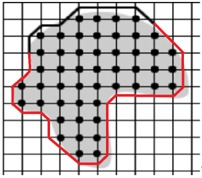
\includegraphics[]{template-FEI/img_01.jpg}\\
    \textbf{a, c, a, b, b, a, b, b, b, c, b, b, b, a, b, a, c, a, b, c, b, a, b, a, c, b}
\end{center}
\vspace{0.5cm}

\noindent\textbf{Questão 04:}

A Figura 3 a seguir corresponde a dois slices de uma Tomografia
Computadorizada, mergulhada em uma subdivisão espacial 3D (representada pelo grid): (a) é o slice no instante $t$ e (b) é o slice no instante $t + 1$. A figura de cubos a seguir a esta contém o mapa de ligações (regras de 1 a 15) pra construção de uma malha triangular 3D da informação (uma cabeça humana). Note os pontos brancos e pretos em alguns voxels. Quando o ponto é preto corresponde a um ponto dentro da informação, quanto é branco, está fora. No mapa de cubinhos, informação do tipo “dentro” é representada por um ponto verde e informação do tipo “fora” não possui ponto algum. RESPONDA: Para cada cubo (base, Figura (a) e topo, Figura (b)) da Figura abaixo, qual a indicação (de 1 a 15) no mapa de cubos da reconstrução?\\
\\
\noindent\textbf{Solução:}

Para os 4 pontos pretos na parte de baixo da figura \emph{(a)} (base) e os 4 pontos brancos na parte de baixo da figura \emph{(b)} (topo), temos a reprodução na \textbf{figura 6}.
\\

Para os 2 pontos pretos e 2 pontos brancos na parte de cima da figura \emph{(a)} (base) e 1 ponto preto e 3 pontos brancos na parte de cima da figura \emph{(b)} (topo), temos a reprodução na \textbf{figura 12}.

\vspace{1cm}
\noindent\textbf{Questão 05:}

Seja o cubo abaixo a esquerda antes da aplicação do Algoritmo de Maching Cubs com a seqüência de indexação sugerida, Index. Qual o valor do índice em binário para cada um dos dois cubos, rotulados cubo 1 e cubo 2, a direita?\\
\\
\noindent\textbf{Solução:}
\[
\textbf{Cubo 1:}
\begin{bmatrix}
0 & 1 & 1 & 1 & 1 & 1 & 1 & 1
\end{bmatrix}
\]
\vspace{0.5cm}
\[
\textbf{Cubo 2:}
\begin{bmatrix}
0 & 0 & 1 & 1 & 0 & 0 & 1 & 1
\end{bmatrix}
\]
\end{document}

